\documentclass[a4paper,12pt]{article}
\usepackage[margin=3cm]{geometry}
\usepackage{setspace}
%\onehalfspacing
\doublespacing
%\usepackage{authblk}
\usepackage{amsmath}
\usepackage{amssymb}
\usepackage{amsthm}

\usepackage[notcite,notref]{showkeys}

\usepackage{psfrag}
\usepackage{graphicx,subfigure}
\usepackage{color}
\def\red{\color{red}}
\def\blue{\color{blue}}
%\usepackage{verbatim}
\usepackage{alltt}
%\usepackage{kotex}

\usepackage{enumerate}

%%%%%%%%%%%%%% MY DEFINITIONS %%%%%%%%%%%%%%%%%%%%%%%%%%%

\def\tr{\,\textrm{tr}\,}
\def\div{\,\textrm{div}\,}
\def\sgn{\,\textrm{sgn}\,}

\def\th{\tilde{h}}
\def\tk{\tilde{\kappa}}
\def\bx{\bar{x}}
\def\bm{\bar{\mathbf{m}}}
\def\K{\mathcal{K}}
\def\E{\mathcal{E}}
\def\del{\partial}
\def\eps{\varepsilon}

\newcommand{\tcr}{\textcolor{red}}
\newcommand{\tcb}{\textcolor{blue}}

\newcommand{\ubar}[1]{\text{\b{$#1$}}}
\newtheorem{theorem}{Theorem}
\newtheorem{lemma}{Lemma}[section]
\newtheorem{proposition}{Proposition}[section]
%\newtheorem{definition}{Definition}[section]
\newtheorem{remark}{Remark}[section]

%%%%%%%%%%%%%%%%%%%%%%%%%%%%%%%%%%%%%%%%%%%%%%%%%%%%%%%%%%
% \usepackage[utf8]{inputenc}

%opening
\title{Second gradient theory, Kinetic model and Thermally driven flow.}
\author{Min-Gi Lee}

\begin{document}

\maketitle

\begin{abstract}

\end{abstract}

This note is, first of all for myself to organize what I read and thought but also for the discussions. I am currently looking into the works of
\begin{itemize}
 \item Yoshio Sone, Kinetic Theory and Fluid Dynamics (2002)
 \item Maxwell(1879), On stresses in rarefied gases arising from inequalities of temperature
 \item Dunn \& Serrin(1984), On the thermomechanics of interstitial working
 \item Giesselmann, Lattanzio, Tzavaras, Relative energy for the korteweg theory and related hamiltonian flows in gas dynamics
 \item Kim, Lee, Slemrod(2015), Thermal creep of a rarefied gas on the basis of non-linear Korteweg-theory
 \item Slemrod(2012), Chapman-Enskog $\Rightarrow$ Viscosity-Capillarity
 \item Karlin \& Gorban(2014), Hilbert's 6th problem : exact and approximate hydrodynamic manifolds for kinetic equations.
\end{itemize}

The current purpose of this note is to address three points.
\begin{enumerate}
 \item I wanted to clarify issues on the signs of terms in the stress come out of the {\it second gradient theory} or {\it kinetic considerations} (Section 5)
 \item One obvious difference between two stress tensors ($T^M$ from kinetic consideration, $T^K$ of korteweg theory) is that the former has the term on $D^2\theta$, $\theta$ the temperature, whereas the latter does not. I want to address that this matters to some extent and clarify the differences and consequences. (Section 6,7)
 \item I certainly can say that in 1D Euler-Korteweg model, Korteweg stress does carry the thermal effect in the correct direction in the presence of the temperature gradient. Its mechanism is to penalize the density gradient and what the korteweg tensor does is to moderate the density gradient and apparently it can be interpreted as the thermal effect. (Section 7)
\end{enumerate}



\tableofcontents

\section{Terminology}
I discriminate the term Thermal creep from thermal stress flow. In a narrow sense, thermal creep is associated to the surface-gas interaction on which the gradient of temperature presences. From hydrodynamic perspective, thermal creep could be modeled only by more elaborate slip boundary conditions. %, we may think of a model without any (thermal) additional stress contribution other than the pressure and the viscosity but with more elaborate boundary conditions that include the slip due to temperature gradient.

On the other hand, the thermal stress is the additional contribution in the stress term in the hydrodynamic model, and Sone refers to the flow purely due to this contribution as the  {\bf thermal stress flow}.

Phenomenologically, we might not able to know where to attribute, however.

Maxwell also distinguished these two, he used the terms normal stress and the tangential stress to denote the stress contribution that are in the normal to the surface boundary. If the surface has uniform temperature, then there will be no tangential stress contribution on the boundary.

\section{Notations}
\begin{itemize}
 \item {{{ $\rho, \theta , \mathbf{v}, T, T^v, T^k$ }}} : density, temperature, velocity, stress tensor, viscous stress tensor, Korteweg stress tensor
 \item $X$ : material coordinate,
 \item $x$ : spatial coordinate,
 \item $x(X,t)$ : motion field, {{{$F_{ij} = \frac{\partial x_i}{\partial X_j}$}}} : deformation gradient, $\tau = det(F) $ : specific volume.
\end{itemize}

\section{Work of Sone}
Idea of Sone : Sone were not concerned with the question of Chapman-Enskog but were concerned with how come we really is able to say some calculations are up to 0th, 1st, 2nd, 3rd ... order of Knudsen number no matter how the approximating system looks like. He refined the asymptotic cases according to the Mach number Ma, and the knudsen number Kn, and named each different expansion by, 1) G-expansion (Grad-Hilbert) 2) S-expansion 3) SB-expansion 4) H-expansion (Hilbert). One crucial thing we bare in mind from his calculation is that-- equations here are pde, and we need some size estimations of the derivatives of the field variables along with the size estimations of fields themselves (w.r.t. Ma and Kn) -- he proceeded the calculation under the size assumption that the differential of a field variable is of comparable size to the field variable. This means he won't probe the short wave for that field. This issue becomes critical in the context of bobylev instability of Burnett and Super-Burnett.

\begin{enumerate}
 \item[Regime 1] Asymptotics around Global Maxwellian 
 \begin{itemize}
  \item Perturbation is assumed to be much smaller than $Kn$ in the leading order and this case corresponds to $Ma, Kn \rightarrow 0$, $Ma \ll Kn$.
  \item He used Linearized Boltzmann equation around the global maxwellian.
  \item He named this expansion as Grad-Hilbert expansion.
 \end{itemize}
 
  \item[Regime 2] Asymptotics around Global Maxwellian
 \begin{itemize}
  \item This case corresponds to $Ma \sim Kn \rightarrow 0$
  \item He used the non-linear Boltzmann equation but from the $Q(f,f)$ terms the linearized part is extracted out explicitly and the residual non-linearity is considered.
  \item He named this expansion as S-expansion
 \end{itemize}
 
  \item[Regime 3] Asymptotics around Local Maxwellian 
 \begin{itemize}
  \item This case also corresponds to $Ma \sim Kn \rightarrow 0$, but the temperature of the Local Maxwellian depends on $x$, the velocity is a perturbation of the uniform velocity.
  \item He used the non-linear Boltzmann equation of the original form.
  \item He named this expansion as SB-expansion
 \end{itemize}
 
  \item[Regime 4] Asymptotics around Local Maxwellian 
 \begin{itemize}
  \item This case corresponds to $Ma \sim O(1)$, $Kn \rightarrow 0$. Both of the temperature and the velocity in the Local maxwellian depend on $x$.
  \item He used the non-linear Boltzmann equation of the original form.
  \item He named this expansion as Hilbert expansion.
 \end{itemize} 

\end{enumerate}

\subsection{remarks of Sone's work}
\begin{enumerate}
 \item In each of expansions, the thermal stress contribution appears in different ways and at different orders. For example, from 1) thermal stress and the slip boundary conditions appear in higher order, from 3) thermal stress appear in the leading order.
 \item Thermal stress flow, or thermal creep flow can occur at different orders in different regimes. For example, from 1) these flow can only be seen at higher order but from 3) flows can be seen from the leading order.
 \item This book is for the steady boundary value problem.
\end{enumerate}


\section{Work of Maxwell}
Maxwell's paper can be summarized as his two assertions and discussions of four different phenomena. What he did is the {\bf Chapman-Enskog} expansion truncated at higher order(Burnett order).

He asserted

 (1) in momentum equation $ \rho \frac{d\mathbf{v}}{dt} = div{T} $,

{{{$$ T = -p \delta_{ij} + T^v + T^M$$}}} and the additional contribution {{{$$T^M = -3\frac{\mu^2}{\rho\theta} \big( D^2 \theta + \frac{1}{2}\Delta \theta\big).$$}}}

 (2) On the solid boundary where temperature gradient exists, the velocity slips and the tangential velocity $u$ is given by

{{{ $$u = G(\rho,\theta) \left[ \frac{\partial u}{\partial x_n} - \frac{3}{2} \frac{\mu}{\rho\theta} \frac{\partial^2\theta}{\partial x_n\partial x_t}\right]  + \frac{3}{4} \frac{\mu}{\rho\theta} \frac{\partial\theta}{\partial x_t},$$ }}}
where $x_n$ and $x_t$ are the normal and the tangential components at the surface, $G(\rho,\theta)$ is a kind of a constitutive relation.
when $G(\rho,\theta)=0$, there is only the tangential temperature gradient contribution.

Maxwell succeeded to explain  the four phenomena with this new contribution. {\it The sign of the contribution was correct to explain the direction of thermal stress in the four phenomena.}  Concerning the bobylev instability at Burnett order, why it was successful despite of the bobylev instability at the Burnett order will be discussed later when I talk about the work of Karlin and Gorban.

\subsection{four phenomena appeared in the paper}
Four phenomena Maxwell discussed are more or less related to the crookes radiometer and after this paper, it seems the there were agreement among the researcher.

\begin{enumerate}
 \item[(A)] temperature on the body is higher (resp. lower) than the ambient temperature. Maxwell said {{{$\theta_{xx}$}}} on $x$-axis has the fixed sign and then there will be an excessive (resp. less) stress on the axis between the bodies, so two bodies repel each other. (resp. attract)
 \begin{figure}[ht]
  \centering
  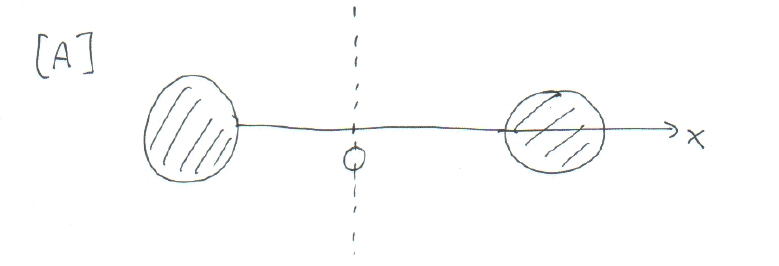
\includegraphics[height=5cm]{Maxwell_A.png}
 \end{figure}
 
 \item[(B)] Cup-shaped body on which temperature is constant. temperature and their derivatives at $p$ is comparable to those with spherical body is placed. On the while, the temperature and their derivatives at $q$ is comparable to those when $q$ is the inside point of the spherical body. This difference makes the stress field non-trivial, and there is the flow (I forgot the direction). 
 \begin{figure}[ht]
  \centering
  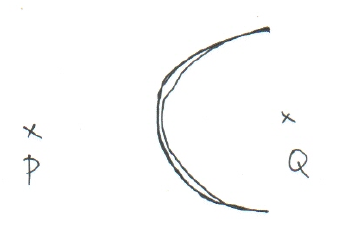
\includegraphics[height=5cm]{Maxwell_B.png}
 \end{figure} 
 Indeed, Crookes came with the cup-shaped radiometer at those times. Even though temperature on both side of the vane is constant, (differently from the standard radiometer setting), this apparatus rotates under the light.
 \begin{figure}[ht]
  \centering
  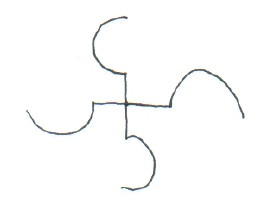
\includegraphics[height=5cm]{cup_radiometer.png}
 \end{figure} 
 
 \item[(C)] Capillary tube on whose boundary temperature gradient presences.

 \begin{figure}[ht]
  \centering
  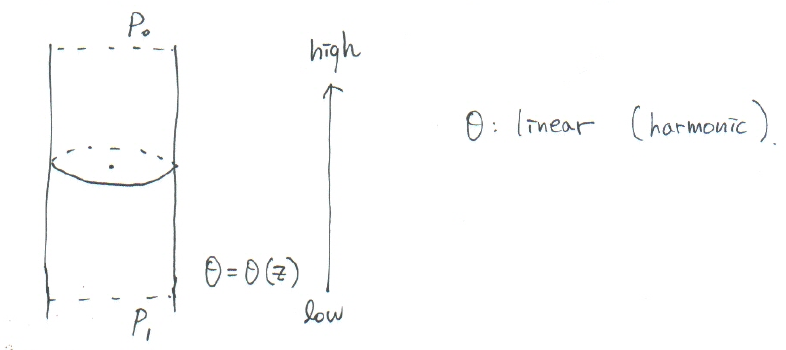
\includegraphics[height=5cm]{Maxwell_C.png}
 \end{figure} 
 It is in the appendix. Here, he approximately calculated and showed that
 \begin{itemize}
  \item If there is no pressure gradient, then net flow is from colder site to the hotter site.
  \item If there is no net flow, then the pressure at hotter site is higher than that of colder site.
 \end{itemize}
It is notable that Maxwell actually performed the approximate calculation of the influence on the pressure-driven flow(poisseulle flow) of the new stress even when the viscosity effect is taken account. Throughout his paper he is saying that, after long time, temperature relaxes to equilibrium (or become harmonic) and if the temperature at the boundary of the domain doesn't have the gradient, then the contribution of {{{$T^M$}}} in the momentum equation vanishes and also pressure becomes constant, which is consistent with the formula of {{{$T^M$}}} above. Speaking of this point, Maxwell pointed out that, when $T^M$ does not contribute and there is no slip at the boundary then there is no way to have the thermal flow in the steady state, insisting that in the thermal creep flow, the slip boundary condition is everything. I'll endeavor this point again later when we consider the Korteweg's stress tensor, not the Maxwell's stress tensor.

 \item[(D)] the standard crookes radiometer
  \begin{figure}[ht]
  \centering
  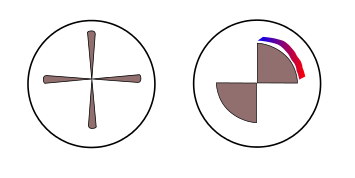
\includegraphics[height=5cm]{2dgeometry.png}
 \end{figure} 

\end{enumerate}

\subsection{remarks of Maxwell's work and discussions}
\begin{enumerate}
 \item All 4 phenomena cannot occur in Navier-Stokes model with no-slip condition.
 \item Maxwell separated issues on assertion (1) on thermal stress and assertion (2) on slip boundary condition. [A] and [B] can be explained without the assertion (2).
 \item There are two ways of demonstration of the presence of the additional contribution in the stress. To make things easier, let's suppose the {\bf temperature is maintained externally} (this amounts to say we ignore the energy equation). The demonstrations depend on what variable other than the temperature we have in our control. Two extremes are found:
 \begin{enumerate}
  \item[(a)] If the {\bf pressure is in our control}, then easiest case is the iso-baric case where the pressure is constant. Then the thermal stress exerts so that there is a flow {\bf from the colder site to the hotter site}.
  \item[(b)] If the {\bf velocity is in our control}, then easiest case is the no flow case where the velocity is $0$. Then the thermal stress exerts so that there is a pressure gradient and {\bf the pressure at the hotter site is greater than that at the colder site.}
 \end{enumerate}

The reasoning is as follows: Suppose there is any additional contribution in the stress term. Then, if we consider the pressure-driven flow (say, the poisseuille flow), the flow behavior is for sure influenced. For simplicity, let us ignore the viscosity for the moment. If no pressure gradient is applied, then for the classical model, there shouldn't be the acceleration. The presence of additional contribution can be demonstrated by showing, there is a non-trivial acceleration even when the pressure is constant. 

The transposition statement of this is : If we don't see any acceleration, then for classical model, pressure has to be constant and the presence of non-trivial pressure gradient implies the presence of the additional contribution in stress.

Then the question, that whether the Korteweg's capillarity theory can also explain the thermal flow or not, is at the {\it direction} of the pressure gradient. The observations of thermally driven flow indicates, the gas flows from colder site to the hotter site. This implies that in the circumstance the flow is absent, the thermal stress is against the pressure gradient or, the pressure at hotter site should be higher. Therefore, in the case (b), the question that the Korteweg theory predicts the thermally driven flow correctly or not boils down to checking whether the pressure increases as temperature increases, and whether the pressure decreases as temperature decreases.

In reality, we may be in the mixed situation where less pressure gradient exists but still is in same direction with the temperature gradient, and less acceleration from the colder site to the hotter site.
\end{enumerate}

\section{Work of Dunn and Serrin}
I didn't summarize the work of Dunn and Serrin. Hoever, the most critical message from this paper in regard to our study is that,
\begin{itemize}
 \item From the free energy function depends on higher gradient of motion and temperature, this paper derives the stress tensor.
 \item It is inconsistent with the Clausius-Duhem inequality, so the authors appended the additional energy flux, the interstitial working.
 \item At the beginning, the stress tensor could have included the terms of $D^2\theta$ because the free energy function depended on higher gradient of the temperature. However, due to the Clausius-Duhem inequality, this possibility is excluded in the course of the stress derivation.
 \item I need to know whether this exclusion is unavoidable or we could have modified theory by making more efforts, as same as they appended the interstitial working term to make the Korteweg tensor be consistent to the Clausius-Duhem inequality. I will read this paper more carefully so that I can answer to this question !
\end{itemize}

\section{Work of Karlin and Gorban, Marshall}
Karlin and Gorban explains the chapman-enskog expansion through the idea of relaxation to the slow manifold regarding the Boltzmann equation as a dynamical system with multiple time scales. In a Boltzmann or other kinetic equation,

{{{$$ \partial_t f + v \cdot \partial_x f = \frac{Q(f,f)}{\epsilon}. $$}}}

\begin{itemize}
 \item From the dynamical system perspective, we treat the field as the field indexed by $v$, $f(v;t,x)=f^v$,
$$ \partial_t f^{v} + Lf^{v} = \frac{Q(f^v,f^v)}{\epsilon}, $$
and view the equation as an infinite dimensional dynamical system. Assuming the suitable integrability conditions, $\{f^v\}_{v\in \mathbb{R}}$ can be expanded to the equivalent infinite number of moments, $(M^0, M^1_{i}, M^2_{ij}, \cdots)$.
 \item Presence of $\epsilon$ in the denominator of r-h-s indicates that the system has the fast-slow structure. To be precise, the nonlinearity $Q(f,f)$ has the kernel, the local Maxwellians, and the set of local Maxwellians is subjected to the template manifold around which the orbits possibly relax.
 \item  The fact that integrals of $Q(f,f)$, $vQ(f,f)$, $|v|^2 Q(f,f)$ vanish, i.e. the 0th moment, first moments, and one second moment vanish, these $5$ variables are not the fast variable but the slow variables. They are $\rho$, $\mathbf{v}$, and $\theta$, the density, velocity, and temperature.
 \item The question is the existence of the {\bf hydrodynamic invariant manifold}, which is around the set of local maxwellians, and on which all other fast components of $f^v$ are determined by the values of the first $5$ moments. 
 
 Note that these moments are in fact fields, with another independent variable $x$. Determinacy here is of functional, for example for a higher moment $M$ that
 $$M = M[\rho,\mathbf{v},\theta]$$
 is a functional dependency upon the $5$ functions that depend on $x$. If, in addition this dependency has a certain {\it locality} restriction in $x$, then we would be able to convert the functional expression into the expression of differential operator
 $$M(x;\epsilon)= \mathcal{M}(\rho(x),D\rho(x),D^2\rho(x), \cdots, \mathbf{v}(x), D\mathbf{v}(x), D^2\mathbf{v}(x), \cdots, \theta(x), D\theta(x), D^2\theta(x), \cdots).$$
 
 The hypothetical picture is that if the field is placed off the manifold then it undergoes the fast relaxation to the hydrodynamic manifold, and the dynamics afterwards is on the manifold, which is the intermediate asymptotics. 
 \item For {\it a given kinetic model}, if we can prove what is said above, then the intermediate asymptotic specify {\it a hydrodynamic model} and we are interested in how the model looks like, or how the stress tensor in the model looks like. 
 
 One important point that this specific hydrodynamic model, which is parametrized by $\epsilon$, would be of the {\it regularly perturbed system}. Whether or not the $M(x;\epsilon)$ has an expansion in $\epsilon$ does not spoil this fact.
\end{itemize}

In the below, I focus on the term $\theta_{xx}$ and its sign and the above issue on regular perturbation with respect to the $\epsilon$.


\subsection{Linearized Grad 13 moments or 10 moments system around the global maxwellian}
This is a brief summary of the paper. The Grad 13 moments or 10 moments system is considered as a given kinetic model, which is parametrized by $\epsilon$ the Knudsen number. The system is linearized around the constant state of $(\rho_0,\mathbf{v}_0,\theta_0)$. From perspective of the Sone's work, this corresponds to his first expansion where Boltzmann equation is linearized around the global maxwellian and there, the interpretation was such that the perturbation size is much less than the Knudsen number. Thus one might be skeptical on the further inference of the results in this line.

\begin{enumerate}
 \item For this linearized system, the hydrodynamic invariant manifold exists, in particular regardlessly of $\epsilon$. However, the expansion in $\epsilon$ fails : high order chapman-enskog exhibit the bobylev instability.
 
 \item The ultimate form of the stress in terms of lower moments in fourier space is
 $$\sigma(k) = - k^2 B(k^2) p(k) - i k A(k^2)v(k),$$
 where $p = \rho + \theta$, (the linearized pressure) and {{{$A(k^2)$}}} and {{{$B(k^2)$}}} are two functions of {{{$k^2$}}} that are negative. So, it is a non-local operator on $p$ and $v$. 
 \item Importantly, this stress does not suffer from the bobylev instability. In the course, the rescale has been done, so in order to invoke $\epsilon$, we need to transform back by replacing $k \mapsto \epsilon k$. 
 \item The functions $A(k^2)$ and $B(k^2)$ are low-pass filters. 
%  
%  Approximately, {{{ $$ A(k^2) \sim -\frac{4}{3 + 9k^2}, \qquad B(k^2) \sim -\frac{4}{3 + 5k^2}. $$ }}}
%  If we invoke $\epsilon$,

Approximately,
{{{ $$ A(k^2) \sim -\frac{4}{3 + 9\epsilon^2 k^2}, \qquad B(k^2) \sim -\frac{4}{3 + 5\epsilon^2 k^2}. $$ }}}
It decays to $0$ as $k^2 \rightarrow \infty$ with tail behavior of $O(\frac{1}{k^2})$.

 \item Marshall presented the entropy dissipation equality for the 10-moments system in the form
$$ \frac{1}{2} \partial_t \int_{-\infty}^{\infty} \frac{3}{5} p(k)^2 + u(k)^2 \; dk + \frac{1}{2} \int_{-\infty}^{\infty} -\frac{3}{5}k^2 B(k^2)p(k)^2 \; dk = \int_{-\infty}^{\infty} k^2 A(k^2) u(k)^2 \; dk, $$
which is consistence in the sense that $A(k^2)$ and $B(k^2)$ are negative. The first term is clearly of classical free energy and the kinetic energy and the second contribution can be interpreted as the {\it non-local capillary} energy.

 \item One can give the heuristic explanation to connect above {\it non-local} to the {\it local} Korteweg type energy. Marshall explained in the paper but I want to refine it as below.  
 \begin{enumerate}
 \item The leading order of $-\frac{3}{5}k^2 B(k^2) \sim -\frac{3}{5}B(0) k^2$
 
 This is the second derivative {\it local} stress with the {\it correct sign}. However the reason why it has the correct sign is rather delicate because in the 13-moments system, it would have a different sign; this reminds us that we do not truncate at the finite order of $\epsilon$ was the main theme.
 \item The reason why the above local leading order has the correct sign is that the bobylev instability of the 10-moments system begins at the Super-burnett order, not from the Burnett order, as can be seen in the paper of Karlin and Gorban. 
 
 \item Without the truncation at the leading order, still we can give the formal explanation to reach the {\it local} version of the stress.
 
 \item For simplicity, let's ignore constants and examine the expression 
 $$b(k^2) = \frac{-1}{1+\epsilon^2 k^2}.$$ A few leading orders of $-k^2b(k^2)$ will be
 $$ k^2(1 - \epsilon^2k^2),$$
 where we see the bobylev instability from the second term.
 \item The expression $-k^2b(k^2)$ is expected to be {\it regularly perturbed}. We can be quite concrete on this. $b(k^2)$ has the inverse fourier transform, which is 
$$ b(\epsilon,x) = \frac{1}{2\epsilon} e^{-\frac{|x|}{\epsilon}} $$
and this kernel has the integral $1$ in entire space. Equivalent way to say that is 
\begin{align*}
 \sigma_{capillary} &= \Delta q, \quad q = (Id - \epsilon^2 \Delta) p, \quad (q(k) = 1+\epsilon^2k^2 p(k)), \quad \text{or}\\
 \sigma_{capillary} &= \Delta(Id - \epsilon^2 \Delta)^{-1} p.
\end{align*}
I remember those expression from Marshall's talk in regard to the failure of truncation of $(I-\epsilon^2 \Delta)^{-1}$. 

\item I did not give any proof, but the above expression formally should converges to $\Delta p$ in {\it a good mode of convergence}.
\item It is true that we would have another $\epsilon$ in front of $\sigma_{capillary}$, so the asymptotic limit as $\epsilon \rightarrow 0$ could be even more trivial. In any sense, this size diminishing, and the convergence to the {\it local} operator are both of {\it regularly perturbed} and the limit of the multiplications of these two also will behave well in my perspective. In addition, the overall size of the capillary stress contribution has to be determined with the problem specification itself, considering non-dimensional quantities, so it has to be separately treated.
\end{enumerate}
\item Now, we come the the local stress $p_{xx} = \rho_{xx} + \theta_{xx}$ that would appear in the limit $\epsilon \rightarrow 0$. Here we have the contribution $\theta_{xx}$ that does not appear in the Korteweg stress tensor. I address this issue because we mentioned that this has incorrect sign in the introduction section of the previous thermal creep paper. After spending some times, my new opinion is that it has the correct sign and that this was the reason why Maxwell succeeded to explain phenomena in his paper. As to the bobylev instability, first of all the instability is the consequence of the eigenvalue analysis for entire linear system rather than the consequence of one term. Besides, it happens when we probe the high frequency functions and other than that it is more or less okay. Recall that Sone either did not take those high frequency functions into account by assuming derivatives of functions are of comparable size to the functions themselves.

\item Regarding to the non-local to local issue, it is worth to look at the approximation Euler-Korteweg model (in Relative Energy paper (2.53)), which was motivated by the numerical concerns.

\item From the form of the kernel 
$$ b(\epsilon,x) = \frac{1}{2\epsilon} e^{-\frac{|x|}{\epsilon}}, $$
it is quite clear why the expansion in $\epsilon$ fails.
\end{enumerate}


\section{Work of Kareem and Min-Gi}
\subsection{difference and similarity between the results of Maxwell's equations of motion and Korteweg's equations of motion}
In order to say the Korteweg theory indicates the correct the thermal behavior, we should be able to predict the phenomena [A] ~ [D]. Even before we consider the radiometer, where the solid boundary has the temperature gradient, we may first go for the cases where surface-gas interaction doesn't quite matter. So, let's focus on the example [A]. [A] can be simplified to 1-D case where the temperature $\theta(x)$ is externally maintained.

%{{attachment:1Dmodel.png}}

We consider the radial symmetric 1-D problem. This can be compared to the case where two hotter (resp. colder) bodies are placed symmetrically at left side and the right side, and this amounts to say we have a control in the temperature distribution, and temperature increases (resp. decreases) in the radial variable $r$. So from the model, we externally assign the temperature as we want. Now, to demonstrate the presence of the thermal stress, we also choose the variable we have in control other than the temperature.

After I read through the Maxwell's paper, I realized the difference of ability in phrasing there is a thermal effect, between the Korteweg model and the Maxwell model.

We want to tell what will happen if one employ the Maxwell's equations of motion or the Korteweg's equations of motion, i.e.

$$ \rho \frac{d\mathbf{v}}{dt} = div(T),$$

Maxwell : {{{ $T = -p \delta_{ij} + T^v + T^M(\rho,\theta)$ }}}

Korteweg : {{{ $T= -p \delta_{ij} + T^v + T^K(\rho,\theta)$ }}}

{{{$$T^M = -3\frac{\mu^2}{\rho\theta} \big( D^2 \theta + \frac{1}{2}\Delta \theta\big).$$}}}

{{{$$ T^K = -\frac{1}{2} \Big[ \rho c_\rho (\rho,\theta) + c(\rho,\theta) |\nabla \rho|^2 + \nabla \cdot \big(\rho c(\rho,\theta) \nabla \rho\big) \Big] \delta_{ij} - c(\rho,\theta) \nabla \rho \otimes \nabla\rho,$$}}} where $c(\rho,\theta)$ is the capillary coefficient.

In 1-D case, and if {{{ $c(\rho,\theta) = c_0 \rho^k \theta^\ell$}}}, then the {{{$T^K$}}} has the following expression {{{ $$ T^k = \frac{c_0}{\alpha} \rho^{\alpha+1} \Big[ \theta^{\ell}(x) (\rho^{\alpha})^\prime \Big]^\prime, \quad \alpha = \frac{k+1}{2} $$}}} which is a non-linear elliptic operator for given $\theta(x)>0$. I'll denote the operator by {{{$ A_\theta[\rho]$}}} and also say $\rho$ is $A$-convex if this is positive and $A$-concave if this is negative.

The question here is the sign and the gradient of {{{$T^M$ (resp. $T^K$)}}} for the given temperature field: Will the gas at the origin feel the excessive stress or restrained stress?

For Maxwell's stress, we can tell the sign of the stress even before we solve the equation, because the temperature is externally given and we can merely calculate the thermal stress directly, whereas for the Korteweg's stress, we don't know the value or sign of this stress until we solve for the $\rho$, which is solved by pde where the temperature appears as the coefficients of the operator. After we have solved for $\rho$, together with $\mathbf{v}$ , we can tell the sign or value of the Korteweg's stress.

The only exception is the iso-baric case, where we put $\rho = 1/\theta$ and we can read off the effect of the Korteweg stress. We examine this case first.

\subsubsection{pressure control}
Suppose we have the pressure in our control, and consider the isobaric case. Then formula {{{$A_\theta[\rho]$}}} amounts to say

{{{ $$ \text{$\theta$ is convex(Maxwell)} \sim \text{excessive stress} \sim  \text{$\theta^{\ell-\alpha}$ is convex, if $\ell>\alpha$ and $\theta^{\ell-\alpha}$ is concave if $\ell<\alpha$  (Korteweg, isobaric)} $$}}}

In view of this, 1) we may say that the Korteweg theory in some sense cause qualitatively similar effect to that of Maxwell, and 2) the sign of Maxwell stress tensor (at Burnett order) is not wrong. (this point is discussed in the section of Karlin and Gorban.)

The disadvantage of the iso-baric case is the stress in general will not be balanced out and there will be acceleration and the non-trivial flow. To have the real solution, we have to solve non-steady mass and momentum equations for $\rho$ and the non-trivial $\mathbf{v}$.

The previous work of Marshall, Yong-Jung and me aimed this demonstration. In this paper we, instead of having temperature externally, assumed the steady state and iso-baric condition. To have self-criticism recalling from now, I should have paid more attention on the boundary conditions on $\rho$ and on the temperature distribution.

\subsubsection{velocity control}
The advantage of this demonstration is that, when the velocity is assumed to be 0, we are only left with the equation of the balance in the stress. $$ div(T) = 0. $$

But as I addressed earlier, the effect of Korteweg stress is rather obscure until we come up with $\rho$. I, at first, was confused for that even this no-flow case can take place.

In addition, let's say if we have some desired direction of the stress {{{$T^K$}}} or the pressure gradient, whether or not it makes physical sense. It seems there is no obstacle to generate such a solution; as $\rho$ re-distribute out rather freely with three boundary conditions, the $\rho$ just seems to adjust as I desire. So, we may be ''design'' the flow in the following order, we fix the temperature -> we fix the desired directional tendency of the pressure -> seek for such $\rho$. From this, I'd like to argue that something does drive the solution in a particular way essentially is the three boundary conditions on $\rho$.

To be concrete, the equation {{{$$ \big(\rho\theta - T^K(\rho,\theta)\big)^\prime = \big( \rho\theta - A_\theta[\rho] \big)^\prime = 0 $$}}} can be manipulated with three boundary conditions of $\rho$ with a lot of degrees of freedom. So if the sign of some quantity is the correctly explaining one for thermal flow, then the boundary conditions play an essential role.

Now, we solve the equation for $\rho$ which is the third order equation.

{{{$$ \partial_x(\rho\theta - T^k) = 0, \quad \text{or} \quad \rho\theta - T^k = T^{total}_0.$$}}}

In this problem,

 * temperature is fixed.
 * Because it is radial symmetric, {{{$\theta^\prime(0) = \rho^\prime(0)=0$, and thus $p^\prime(0)=0$.}}}
 * {{{$\rho(0)= \rho_0$}}}
 * The the total stress {{{$T^{total}_0$}}} is an undetermined constant. If this were known, then the {{{$\rho^{\prime\prime}(0)$}}} could have been known and also the sign of the Korteweg stress could have been known. This could be measured at the boundary $x=L$ or at far field according to the problem setting, but in order to solve the equation in the setting of initial-value problem, we specify the constant first and shoot the ode playing with the two parameters {{{$\rho_0$}}} and {{{$T^{total}_0$}}}.

Our statement for the Korteweg's equations of motion is the dichotomy,

 1. for given two parameters {{{$\rho_0$}}} and {{{$T^{total}_0$}}}, the shot solution does not survive to exist until $x=L$.

 1. the shot solution does exist and the pressure increases in $[0,L]$.

We verify the statement first numerically, using ode solver(Runge-Kutta) in python.

First of all, in the increasing-temperature case, the case {{{$T^{total}_0<0$}}} is not very interesting because : If so, initially $\rho$ is accelerated and being {{{$T^{total}_0<0$}}} and increasing temperature make this acceleration bigger and bigger. No doubt for pressure increase. (in the decreasing-temperature case, same applies for {{{$T^{total}_0>0$}}})

Kareem and I ran many instances. The overall behavior seen from the calculations is,

 1. pressure gradient direction always is in correct direction.

 1. If the reference scale of the temperature is quite bigger than that of $\rho$ (like 10 times bigger), then the variation of $\rho$ seems to be suppressed, in other words, in the pressure $p=\rho\theta$, $\rho$ does not re-distribute out against the temperature gradient.

I put increasing-temperature case and decreasing-temperature case in the below.

%{{attachment:lorentzdist-inc.png||height="300",width="300"}} %{{attachment:parabola-dec.png||height="300",width="300"}}

\section{Isothermal capillary problem vs. thermal-stress flow problem}
Here, I want to demonstrate the similar structure observed in the 1D case between the isothermal capillary problem and the thermal-flow problem.

In the capillary problem, let's consider the gravity in $z$-direction and assume there is no flow($\mathbf{v}=0$). If we are to use Korteweg stress tensor, then in the stress balance,

{{{$$\partial_z(-\rho\theta_0 + T^K) = -1$$}}} {{{$$-\rho\theta_0 + T^K = -z + const.$$}}}

Hence, we have an elliptic operator

{{{$$-T^K = -A[\rho] = -(\rho +z) + const., \quad \text{where $A_{\theta_0}[\rho]$ is an elliptic operator defined above, and I set $\theta_0=1$} $$}}}

In the thermal-stress problem, {{{$$\partial_z(-\rho\theta(z) + T^K) = 0$$}}}

Hence, we have an elliptic operator

{{{$$-T^K = -A_\theta[\rho] = -\rho\theta(z) + const., \quad \text{where $\theta(z)$ is an increasing function of $z$} $$}}}

As long as $\theta(z)>0$, the left hand side is non-linear elliptic operator. The right-hand-side in the capillary problem and the thermal-stress problem have different reaction and source term but might imply shared property.

\section{Hamiltonian structure and dissipative structure of isothermal and non-isothermal Euler-Korteweg model}
In the Euler-Kortweg model, we put the helmholtz energy functional

{{{ $$ \mathcal{E} = \int h(\rho,\theta) + \frac{1}{2}\kappa(\rho,\theta) |\nabla\rho|^2 \, dx $$ }}}

In the iso-thermal case, Euler-Korteweg model is hamiltonian system. In the paper of Jan and Thanos, they mentioned about the Benzoni-Gavage's hamiltonian formulation which is valid only when the curl of $\mathbf{v}$ vanishes, but as they remarked, the hamiltonian is better looked as a function of the generalized coordinate and the generalized momenta rather than the function of $\rho$ and $\mathbf{v}$.

I'll fill in the calculation gaps in the below later on, but it should have natural hamiltonian system structure with hamiltonian depending on the motion and the momenta $(x(X,t), \mathbf{m}(X,t))$.

----
Following the serrin's book(mathematical principles of classical fluid mechanics), first consider the hamiltonian functional in the material coordinate $X$ and write the density {{{$\rho J = \rho_0$}}}, where $J$ is the determinant of the deformation gradient. I purposely exposed the constant {{{$\rho_0$}}} rather than using $1$. Formal calculation gives

{{{ $$ H = \int \frac{1}{2} \rho|\mathbf{v}|^2 + h(\rho,\theta) + \frac{1}{2}\kappa(\rho,\theta) |\nabla\rho|^2 \, dx $$ }}}

{{{ $$ H = \int \rho_0(X) \left(\frac{1}{2} |\mathbf{v}|^2 + \tilde{h}(\rho) + \frac{1}{2}\tilde{\kappa}(\rho) |\nabla_{x}\rho|^2\right) \, dX, $$ }}} we set {{{$\mathbf{m} = \rho_0(X)\mathbf{v}$, $\tilde{h}(\rho) = h(\rho)/\rho$, $\tilde{\kappa}(\rho)= \kappa(\rho)/\rho$}}}.

{{{ $$ H(x(X,t),\mathbf{m}(X,t)) = H(\rho(X,t),\mathbf{m}(X,t)) = \int \left(\frac{1}{2\rho_0(X)} |\mathbf{m}|^2 + \tilde{h}(\rho) + \frac{1}{2}\tilde{\kappa}(\rho) |\nabla_{x}\rho|^2\right) \, dX $$ }}} Hamiltonian system is {{{ $$\frac{dx(X,t)}{dt} = \frac{\delta H}{\delta \mathbf{m}} = \frac{\mathbf{m}}{\rho_0(X)} =  \mathbf{v}  $$}}} {{{ $$\frac{d\mathbf{m}(X,t)}{dt} = -\frac{\delta H}{\delta x} $$}}}

----
When the flow is non-isothermal, Euler-Korteweg system is dissipative with modification of Dunn \& Serrin. (I'll more endeavor to understand the procedure)
\end{document}
